\documentclass{report}

\usepackage[utf8]{inputenc}
\usepackage{natbib} % to use bibliography
\usepackage{graphicx} % to include graphics
\usepackage{subcaption} % to include sub graphics
\usepackage{amsmath} % to include extended mathematics
\usepackage[breaklinks]{hyperref} % to include links
\usepackage[acronym, toc]{glossaries} % to include a glossary
\usepackage{fancyhdr} % to style header and footer
\usepackage[nottoc]{tocbibind} % adds bibliography to ToC
\usepackage{listings} % to include code snippets
\usepackage[table]{xcolor} % to colorize source code and table cells
\usepackage{array} % to define custom column types
\usepackage{multicol} % to create lists with multiple columns
\usepackage{multirow} % to create lists with multiple rows

% define column types with a fixed length
\newcolumntype{L}[1]{>{\raggedright\let\newline\\\arraybackslash\hspace{0pt}}m{#1}}
\newcolumntype{C}[1]{>{\centering\let\newline\\\arraybackslash\hspace{0pt}}m{#1}}

% set resources path
\graphicspath{ {./resources/} }

% create hyperlinks for ToC
\hypersetup{
    linktoc=all,
}

% define colors for code
\definecolor{commentsColor}{rgb}{0.497495, 0.497587, 0.497464}
\definecolor{keywordsColor}{rgb}{0.000000, 0.000000, 0.635294}
\definecolor{stringColor}{rgb}{0.558215, 0.000000, 0.135316}

\lstset{ %
  backgroundcolor=\color{white},   % choose the background color
  basicstyle=\ttfamily\footnotesize,        % the size of the fonts that are used for the code
  breakatwhitespace=false,         % sets if automatic breaks should only happen at whitespace
  breaklines=true,                 % sets automatic line breaking
  captionpos=b,                    % sets the caption-position to bottom
  commentstyle=\color{commentsColor}\textit,    % comment style
  deletekeywords={...},            % if you want to delete keywords from the given language
  escapeinside={\%*}{*)},          % if you want to add LaTeX within your code
  extendedchars=true,              % lets you use non-ASCII characters; for 8-bits encodings only, does not work with UTF-8
  frame=tb,	                   	   % adds a frame around the code
  keepspaces=true,                 % keeps spaces in text, useful for keeping indentation of code (possibly needs columns=flexible)
  keywordstyle=\color{keywordsColor}\bfseries,       % keyword style
  language=Python,                 % the language of the code (can be overrided per snippet)
  otherkeywords={*,...},           % if you want to add more keywords to the set
  numbers=left,                    % where to put the line-numbers; possible values are (none, left, right)
  numbersep=5pt,                   % how far the line-numbers are from the code
  numberstyle=\tiny\color{commentsColor}, % the style that is used for the line-numbers
  rulecolor=\color{black},         % if not set, the frame-color may be changed on line-breaks within not-black text (e.g. comments (green here))
  showspaces=false,                % show spaces everywhere adding particular underscores; it overrides 'showstringspaces'
  showstringspaces=false,          % underline spaces within strings only
  showtabs=false,                  % show tabs within strings adding particular underscores
  stepnumber=1,                    % the step between two line-numbers. If it's 1, each line will be numbered
  stringstyle=\color{stringColor}, % string literal style
  tabsize=2,	                   % sets default tabsize to 2 spaces
  title=\lstname,                  % show the filename of files included with \lstinputlisting; also try caption instead of title
  literate={\ \ }{{\ }}1,
  columns=fixed                    % Using fixed column width (for e.g. nice alignment)
}

% rename bibliography to references
\renewcommand{\bibname}{References}

% define header and footer
\pagestyle{fancy}
\fancyhf{} % clear all
\renewcommand{\chaptermark}[1]{\markboth{#1}{}}
\renewcommand{\sectionmark}[1]{\markright{#1}}
\lhead{\rightmark}
\rhead{\textbf{\leftmark}}
\cfoot{\thepage}

\title{\textbf{Nero} - Named-Entity Recognition for Swiss Mobiliar}
\author{Yves Beutler}
\date{January 2020}

% initialize glossary
% \makeglossaries
% \newglossaryentry{mobi24}
{
    name=mobi24,
    description={the 24h assistance and emergency call center of Swiss Mobiliar}
}

\newglossaryentry{infomobi}
{
    name=infomobi,
    description={mailbox from info@mobiliar.ch used as data source}
}

\newglossaryentry{meinemobi}
{
    name=meinemobi,
    description={mailbox from meinemobiliar@mobiliar.ch used as data source}
}

\newglossaryentry{Duden}
{
    name=Duden,
    description={a spelling dictionary of the German language}
}

\newglossaryentry{diacritic}{
    name=diacritic,
    description={a sign added to a letter to indicate a different pronunciation}
}

\newglossaryentry{Protekta}
{
    name=Protekta,
    description={the legal protection insurance which is part of Swiss Mobiliar}
}

\newacronym{ner}{NER}{named-entity recognition}

\newacronym{nlp}{NLP}{natural language processing}

\newacronym{ml}{ML}{machine learning}

\newacronym{iob}{IOB}{Inside-outside-beginning}

\newacronym{pst}{PST}{Personal Storage Table}

\newacronym{kpi}{KPI}{key performance indicator}

\newacronym{ne}{NE}{named entity}

\newacronym{rnn}{RNN}{recurrent neural network}

\newacronym{dnn}{DNN}{deep neural network}

\newacronym{bfh}{BFH}{Bern University of Applied Sciences}

\newacronym{mlp}{MLP}{multilayer perceptron}

\begin{document}

\maketitle

\tableofcontents
\listoffigures
\listoftables
% \lstlistoflistings

% insert chapters here
\chapter{Introduction}

Natural language processing (\acrshort{nlp}) is a subfield of linguistics, computer science, and artificial intelligence dealing with the interaction between computers and humans using natural language. \acrshort{nlp}s main objective is to decipher, interpret, and react to human language which often relies on \acrlong{ml} techniques. Natural language includes both speech and text \cite{garbade}. There exist many use cases for \acrshort{nlp} such as text-to-speech transformation, machine translation\footnote{Translating one written language into another like Google Translator or DeepL does}, part-of-speech tagging\footnote{The process of identifying nouns, verbs, adjectives, adverbs, etc.}, and \acrlong{ner}. This bachelor thesis is about the latter topic, also called \acrshort{ner}.

\section{Project Overview}

\Gls{mobi24} is an assistance and emergency call centre founded by the Swiss Mobiliar in 1997. It's the initial contact point for clients and potential future clients. Most of the in-going requests are insurance related subjects. The purpose of this bachelor thesis is the creation of a natural language model for \acrlong{ner} in the insurance context based on client data from \gls{mobi24}. There already exist several pretrained models which are free to use, but just a few of them are capable of dealing with the German language and none of them are trained with insurance data. In the future, the model from this thesis should help the data scientists at Swiss Mobiliar for their own specific \acrshort{nlp} tasks. Currently the most interesting named entities for Swiss Mobiliar are the people's names and their addresses. Consider chapter \ref{chap:ner-overview} for detailed information about \acrshort{ner} and how it works.

\subsection{Objectives}

For a successful completion of the bachelor thesis several deliverables need to be offered to the stakeholders. Additionally to this document there should exist a functioning language model with an anonymised training data set. This training set should have an appropriate size for training the model and comparing the different outcomes. The source code should be written under consideration of the commonly known software engineering and design patterns. The model is developed iteratively with one or more baseline models\footnote{A very simple approach which sets the minimal requirements for NER} at beginning. The goal is to optimise the model with every new approach to get the most accurate output possible.

From an administrative point of view there are several deliverables this bachelor thesis has to provide. A summarized overview about all objectives can be found in the table below. Consider table \ref{tbl:deadlines} for the corresponding deadlines.

\begin{enumerate}
    \item \acrshort{ner} model (with anonymised training / validation data)
    \item Bachelor thesis (current document)
    \item Presentation for the \acrshort{bfh} techdays 2020
    \item Abstract for the \acrshort{bfh} publication of all bachelor theses
    \item Poster (of size A3)
    \item Short movie clip about the project's essentials
\end{enumerate}

\subsection{Submission Deadlines}

This bachelor thesis is carried out in compliance with various deadlines. Table \ref{tbl:deadlines} gives an insight about the most relevant milestones and when they should be delivered to the stakeholders.

\begin{table}[ht!]
    \centering
    \begin{tabular}{|l|l|}
        \hline
        \textbf{Date} & \textbf{Submissions and Milestones} \\ [0.5ex]
        \hline
        16.09.2019 & Begin of semester, project kick off \\
        03.01.2020 & Submission of poster (A3) \\
        16.01.2020 & Submission of report, movie clip \\
        17.01.2020 & Presentation at BFH Techday \\
        17.01.2020 & Poster exhibition \\
        07.02.2020 & Grading conference \\
        06.03.2020 & Graduation party \\ [1ex]
        \hline
    \end{tabular}
    \caption{Most important (submission) dates}
    \label{tbl:deadlines}
\end{table}

\subsection{Stakeholders}

There are several stakeholders interested in the outcome of this project. There is the Swiss Mobiliar and especially its data scientists, who want to reuse the trained \acrshort{nlp} model for their own projects. On the other hand, there is the \acrlong{bfh} which is demanding a satisfactory thesis for awarding me with the bachelor's degree in computer science. Last but not least, I act as a stakeholder as well and I want to dig deeper in the field of data science and learn as much as possible.

It will be challenging to satisfy all these different stakeholders to an adequate level. Swiss Mobiliar is very focused on the resulting model whereas the \acrshort{bfh} is more interested in the overall project, including time and project management.

\section{Organisation}

This bachelor thesis is written during my last semester at the \acrlong{bfh} while I'm working full-time at the Swiss Mobiliar in the Department of \emph{Cognitive Computing \& Disruptive Analytics}. The department is mainly responsible for the development of cognitive applications to support existing business processes. The team is also driving the digital transformation and making Swiss Mobiliar data addicted.

\subsection{Coordination}

Swiss Mobiliar is working with the \emph{Atlassian} tool stack. \emph{Jira} is used for keeping track of all tasks and dealing with bug requests. The Kanban boards model the current project state by visualising the progress of each story or task.

I'm a member of the agile Scrum team \emph{Aare}\footnote{The beautiful river called Aare floats through the city of Berne}. Due to the Scrum methodology, my colleagues are getting informed about my progress every morning at the daily scrum. At the end of each sprint\footnote{At Swiss Mobiliar a sprint has a total duration of 3 weeks}, there is a Scrum activity called \emph{Sprint Review} where I present my latest findings to the team.

\begin{figure}[!ht]
\centering
\frame{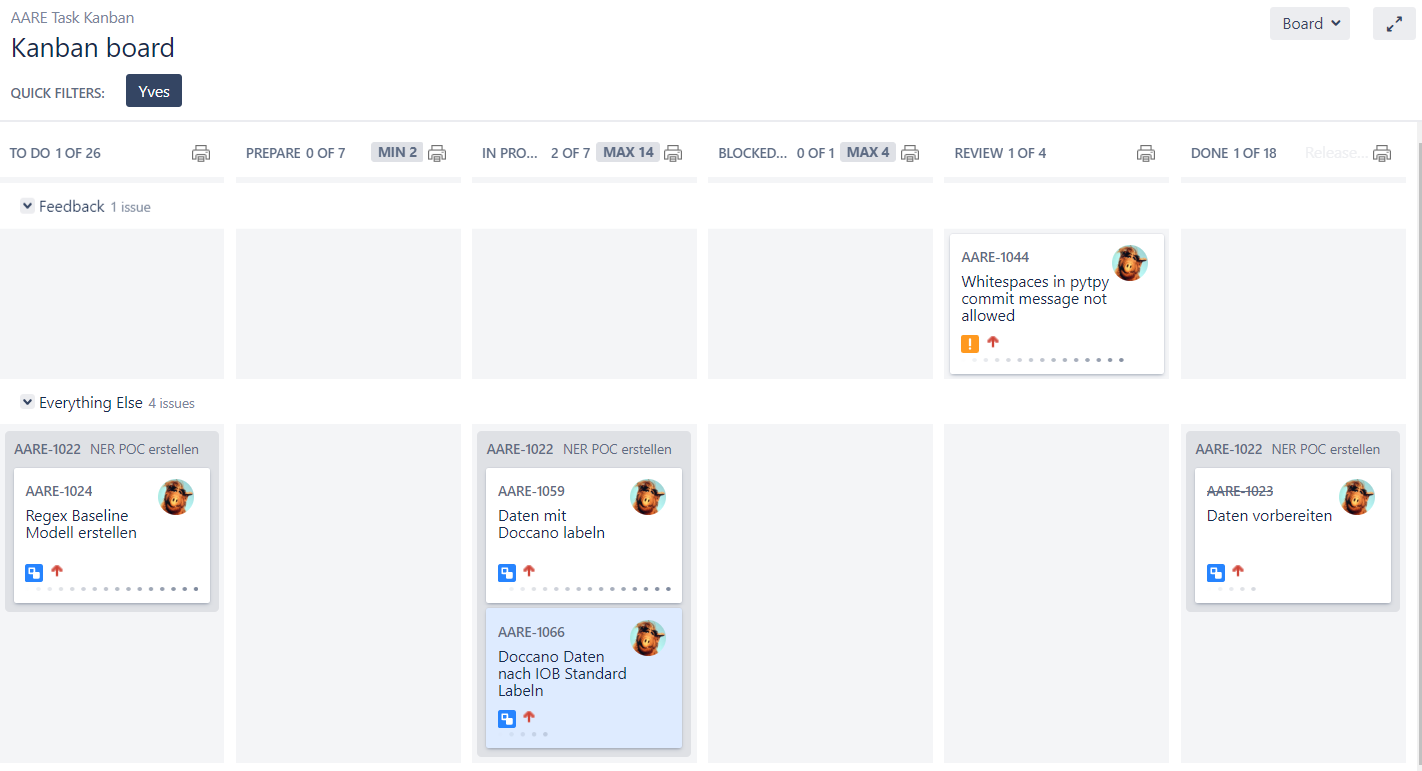
\includegraphics[width=\textwidth]{kanban}}
\caption{View of the Kanban board at an early project stage}
\label{fig:kanban}
\end{figure}

My supervising professor and I organise an informal meeting roughly every two weeks to discuss the project progress and to plan the next steps. During this session I've got the time to ask questions concerning my current tasks. Due to the short time span between these meetings, the project itself becomes very agile. I am able to change my primary focus to a different task within weeks.

\subsection{Development Environment}

All source code is generally written in Python. Small code snippets, mostly for exploring and mapping data into another structure, are created with \emph{jupyter notebooks}. The models and larger pre-processing steps need to be robust and comprehensible, so unit tests must be created. This code is under version control and is pushed frequently to the internal Git repository of Swiss Mobiliar. Teamcity is used as a build server, which controls and deploys the code as a python library. To simulate later applications, the model code is being run inside a docker container\footnote{Tool to run applications inside a container independent of the underlying operating system}.

\section{Data Privacy Declaration}

All used examples and data snippets in this document are anonymised to protect the privacy of Swiss Mobiliar's clients. All names and addresses are either cropped out of the original text or purely fictional. The training and validation data given to the supervising professor for validating the final model is anonymised too.

\chapter{Fundamentals}
\label{chap:ner-overview}

This chapter aims to give the reader a basic overview about the idea behind \acrlong{ner}, the expected benefits for Swiss Mobiliar, and information about the state of the art. General difficulties and the solutions to these problems are mentioned as well.

\section{A Brief Overview}

\acrshort{ner} is a subtask of information extraction. It seeks to find named entities (\acrshort{ne}) in unstructured text and classify them into predefined categories such as person names, locations, and organisations. A \acrlong{ne} is a real-world object with a proper name like \emph{Roger Federer}, \emph{New York City}, or the \emph{catholic church} \cite{wiki02}. Table \ref{tbl:named-entities} shows typical \acrlong{ne} types which are supported by a large variety of \acrshort{ner} libraries. Sometimes this group is extended with types like prices, dates, and times \cite{Jurafsky2000}. It's common to create own domain specific entities, e.g. an entity type \emph{insurance} which might be useful for the Swiss Mobiliar. Locations and geo-political entities are sometimes combined\footnote{The NLP library spaCy combines these two for models trained with the Wikipedia corpus}.

\begin{table}[h!]
    \centering
    \begin{tabular}{|l|l|l|}
        \hline
        \textbf{Type} & \textbf{Tag} & \textbf{Description} \\ [0.5ex]
        \hline
        People & PER & People, Characters \\
        Organisation & ORG & Companies, NGOs, Sports \\
        Locations & LOC & Regions, Mountains, Seas \\
        Geo-Political Entity & GPE & Countries, Cities, Provinces \\ [1ex]
        \hline
    \end{tabular}
    \caption{List of generic named entity types}
    \label{tbl:named-entities}
\end{table}

Due to the different language structures a \acrshort{ner} model only fits to the language(s) it's build for. These hasn't to be only national languages. This could possibly be business, sports, or in this reports case, insurance language.

There are two main approaches for \acrlong{ner}: A rule-based or a statistical system. The rule-based \acrshort{ner} uses a ruleset trying to define the characteristics of a language. Language as well as the appearance of named entities follow specific patterns. In German for example, names are always written in uppercase. Therefore a simple regular expression\footnote{Pattern for defining character sequences used for search, replace or validation operations} will help recognising \acrshort{ne}s of type name. Needless to say, that the rule doesn't catch misspelled names.

The statistical \acrshort{ner} instead is based on probabilities. When dealing with a high term ambiguity or with a giant vocabulary, the statistical approach is often more reasonable \cite{blub}. The ruleset of a rule-based system will grow along with an increasing vocabulary, which makes maintaining the model very difficult. How a statistical \acrlong{ner} works and what deep learning exactly is, will be explained at a later point.

\section{Use Cases}

A reasonable \acrshort{ner} model will give the Swiss Mobiliar several benefits in understanding natural language and thereby offering an even better service to its customers. The model will be available as a python library in the Swiss Mobiliar repository so that data scientists can use it in their own projects. Due to limited time resources the final model will only recognise names and addresses. However, it's possible to extend the list of named entities with new values like phone numbers or insurance polices.

\subsection{Automated Tagging}

A very common use case for \acrlong{ner} is the automated tagging of articles, web pages, or documents. A news provider could recommend related articles with the same tagged entities to its readers. Furthermore search algorithms profit from tags as well. Imagine the performance benefits of searching over a million tags instead of a million document bodies \cite{gupta}. Swiss Mobiliar could use the \acrshort{ner} for clustering its large sets of \emph{confluence} articles into specific groups.

\subsection{Reduced Complexity}

One main advantage is to reduce the amount of distinctive words in the data. This set of words is called vocabulary. The German vocabulary consists of 300 000 to 500 000 tokens according to various sources \cite{wiki03}. The larger the vocabulary, the larger a deep learning model needs to be to comprehend the language. A bigger model is larger in size and needs more time to train. The size of a deep learning model can be measured by the number of parameters it has. This is called parameter space. The parameter space defines how a deep learning model adapts to data. Very few parameters may not be enough to learn more complex patterns. Too many parameters and the model doesn't need to generalise because it can memorise mostly everything.

\begin{table}[h!]
    \centering
    \begin{tabular}{|l|c|c|c|c|c|c|c|}
        \hline
        \textbf{Default} & Sherlock & Holmes & lives & at & 221b & Baker & Street. \\
        \hline
        \textbf{Reduced} & PER & lives & at & LOC & & & \\
        \hline
    \end{tabular}
    \caption{Comparison of two sentences}
    \label{tbl:param-space}
\end{table}

Table \ref{tbl:param-space} illustrates how the \acrshort{ner} can minimise the vocabulary size of a given data set. While the origin sentence has a vocabulary of size 7, the reduced sentence only consists of 4 tokens. It uses $\frac{4}{7}$ of the tokens to express nearly the same amount of information. The parameter space can be decreased for smaller vocabularies. This results in better model performance. Especially if you want to develop micro services, a lightweight and therefore fast model is required to satisfy customers needs.

\subsection{Anonymisation}

It's important to keep in mind that real anonymisation isn't possible. After data is being de-identified\footnote{The process of anonymising personal data} it can be used and shared without the restrictions of data protection laws. Sharing research data across institutions boosts the development of scientific inventions. The problem is that the data only seems to be anonymised. In fact, there is a high chance to recognise individuals if the data is being populated with additional data sources \cite{rocher19}. Imagine a de-identified insurance case about a car accident. There's the possibility to simply search news sites for car accidents at the concrete date to get personal information about the vehicle type or even the owner.

Nevertheless, the \acrshort{ner} model will be used to create anonymised data. The anonymised data could be used for demonstration purposes. Even training in a cloud-based infrastructure would be significantly easier because of less restrictions from data policies. All data processed by the \acrshort{ner} model can be freely distributed across Swiss Mobiliar.

Instead of removing personal information there is also the opportunity to replace named entities with fictional values. The data would look correct but isn't mirroring the reality and thus can be shared again. Although this approach may confuse users which aren't aware of the fact that the entities are fictional it's worth mentioning. An advantage is that if a \acrshort{ne} was not recognised and anonymised, the user would not know.

\subsection{Form Completion}

In information extraction, such a model can be useful to localise user data and complete a form with the extracted parts. If you combine the model with an intent classifier\footnote{A model to predict user intents, widely used in smart assistants}, a very powerful combination arises \cite{jain18}. You could create pre-filled insurance offers from client requests. This would speed up the process and may result in more sales. Swiss Mobiliar is currently doing research on chat bot for assisted claims management, including damage classifier and automated suggestions.

\section{State of the Art}

Latest \acrshort{ner} models achieve f1-scores of 93.5\% on the \emph{CoNLL-2003} dataset \cite{art19}. The f1-score is a performance indicator which considers both the precision and recall to compute the score. The \emph{CoNLL-2003} dataset contains part-of-speech tags next to \acrlong{ne} tags and is the standard dataset to test \acrshort{ner} model performances. Consider section \ref{chap:formulas} for more information on performance measures.

The \acrshort{nlp} model for achieving nowadays highest results is called \emph{BERT} \cite{bert18}. Developed by Google and released in 2018, \emph{BERT} sets new standards for \acrlong{nlp} tasks. Unlike previous models, \emph{BERT} uses the context before and after a word to describe its meaning. For more information about \emph{BERT}, have a look at the repository hosted on Github \cite{bert-gh}.

Despite the good results of current \acrlong{ml} models, people perform still better in recognising \acrshort{ne}s. According to the \emph{MUC-7}\footnote{Message Understanding Conference, which took place in 1997}, human annotators scored more than 97\% \cite{wiki04}. 

\section{Difficulties in Processing Natural Language}

In \acrlong{ner} it can be very difficult to decide what's a named entity and what's not. The term \emph{general agency Berne} can refer to an organisation whereas the token \emph{Berne} could reference the capital of Switzerland. For the best possible results it's important to define the boundaries of what's a named entity and what's not and to be strict while labelling.

Another difficulty is if you have to deal with word ambiguity. Imagine the entity \emph{Orange} which can either be a fruit, a colour, a telecommunication provider or a city in France. Many fashion labels are named after designers like \emph{Calvin Klein} or \emph{Ralph Lauren} but when people mention them, they mostly mean the brand rather than the actual person \cite{Vogel19}. The \acrshort{nlp} model needs to consider the context in which the ambiguous term occurred to give a solid prediction.

\section{Performance Measurement}
\label{chap:formulas}

There exist several performance indicators each data scientist should be aware of. These specific metrics are used to validate the outcome of models and make different solutions comparable. As in figure \ref{fig:metrics} displayed, there is a basic concept which these metrics are build on top of.

\begin{figure}[!ht]
\centering
\frame{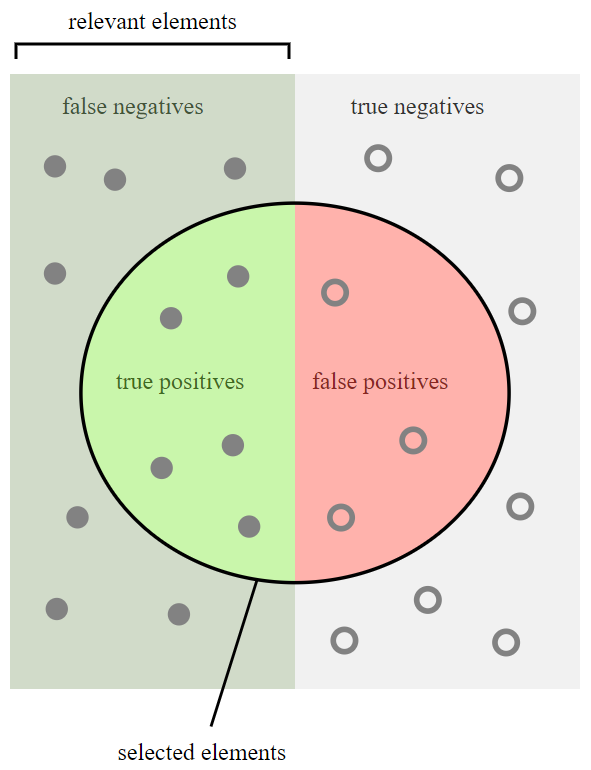
\includegraphics[scale=0.4]{metrics-overview}}
\caption{Overview about possible classification outcomes\cite{wiki01}}
\label{fig:metrics}
\end{figure}

For every binary classification task there exist exactly four possible outcomes. When the model classifies an element correctly it's either a \emph{true positive} or a \emph{true negative} value. The keyword true relates to the prediction the model did. Vice versa it's either a \emph{false positive} or a \emph{false negative} value if the model's prediction is wrong.

The combination of \emph{true positive} and \emph{false negative} values is the amount of relevant data we want to have a closer look at. For example this could be a set of named entities or a group of patients which have a certain disease.

\subsection{Why Accuracy is not enough}
\label{chap:accuracy}
Probably the most well-known and certainly the easiest metric to understand is called \emph{accuracy}. It describes the
closeness of a set of predictions to its corresponding \emph{truth values}. Accuracy is the proportion of all correctly classified
elements in relation to the total quantity. It's value lies somewhere between zero and one.

\begin{equation}
    \label{math:accuracy}
    accuracy = \frac{\textit{true positives} + \textit{true negatives}}{\textit{total population}}
\end{equation}

There is one large downside with accuracy which makes it useless for many classification problems. If there's one category
representing the majority of elements, accuracy will always be at a very high level. This is called an \emph{imbalanced
classification problem} \cite{koehrsen}. Imagine a model for detecting very rare diseases which simply labels each tested patient
as \emph{negative}. If the chance of getting this disease is about \(\frac{1}{10000}\), the accuracy of such model would be at
stunning $99.99\%$. That's why every data scientist should consider using more advanced metrics as described in the next section.

\subsection{Precision and Recall}

\emph{Precision} measures the accuracy of the positive predictions. In other words, it's the proportion of correctly classified
elements in relation to all elements the model marked as \emph{positive}. A model which classifies only one single element as
\emph{positive} (the rest as \emph{negative}) and is right about that, will have a \emph{precision} of $1.0$. The results of a
model with a high \emph{precision} are very useful because most values have been correctly classified and therefore can be used
for further processing.

\begin{equation}
    \label{math:precision}
    precision = \frac{\textit{true positives}}{\textit{true positives} + \textit{false positives}}
\end{equation}

\emph{Recall}, or sometimes called \emph{sensitivity}, is the number of correct classifications compared to the number of elements
which should have been found in total. A \emph{recall} of $100\%$ can simply be achieved by classifying every element as \emph{positive}.
Therefore it should be combined with \emph{precision} to get an expressive statement about the model performance.

\begin{equation}
    \label{math:recall}
    recall = \frac{\textit{true positives}}{\textit{true positives} + \textit{false negatives}}
\end{equation}

There is a trade-off between the two metrics \emph{precision} and \emph{recall}. An optimization which increases the \emph{recall}
will likely decrease the \emph{precision} and vice versa. If neither \emph{recall} nor \emph{precision} is more important, there
exists the \emph{F1 score} (\ref{math:f1}) which is the harmonic mean of both. The mean itself isn't very meaningful because if the
model performs very good at one metric and poorly at the other, it will be still around $0.5$. The harmonic mean punishes low values
and doesn't compensate them with high values for the opposite metric. In many cases, \emph{F1 score} is a good metric to describe the
overall performance of a model \cite{Grus15}.

\begin{equation}
    \label{math:f1}
    \textit{f1 score} = 2 * \frac{precision * recall}{precision + recall}
\end{equation}


\chapter{Preprocessing}

Data preparation takes 60 to 80 percent of the whole analytical pipeline in a typical machine learning project. It's very important to get an overview about the data before starting to build up a model. This seems to be a lot of time and effort, but will save you a lot of time afterwards \cite{naman18}. In many machine learning projects preprocessing is the most important part. A solid data basis can increase the performance of the model. Furthermore, preprocessed data is much more comfortable to deal with than raw data.

\section{Data Sources}
\label{chap:data-source}

The NLP model relies on two distinctive data sources. In detail, there is a single \emph{Personal Storage Table (PST) \footnote{An open proprietary file format by Microsoft used to store copies of messages}} for the email mailboxes \emph{info@mobiliar.ch} and \emph{meinemobiliar@mobiliar.ch}. For a better understanding, the two data sources are called \emph{infomobi} and \emph{meinemobi}. \emph{infomobi} is the single point of contact for every Swiss Mobiliar related question or request, whereas \emph{meinemobi} is only used by the clients of the \emph{"Meine Mobiliar"} customer platform. The platform gives you an overview of your active policies or lets you report a claim.

Both data sets contain email messages in three different formats. The most commonly used kind is \emph{HTML}, followed by some \emph{Plain Text} and even fewer \emph{RTF} messages.

\begin{figure}[!ht]
    \centering
    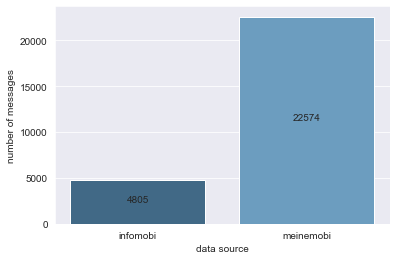
\includegraphics[scale=0.5]{plot-comparison-size}
    \caption{Size comparison of both data sources}
    \label{fig:plot-comparison-size}
\end{figure}

Figure \ref{fig:plot-comparison-size} shows, that the size of \emph{meinemobi} is more than four times larger than the size of \emph{infomobi}. Before pre-processing there is a total number of 27 379 messages. This is a solid base if we keep in mind, that a large part of the data may be removed at data cleansing. Afterwards, the remaining data needs to be labelled manually to build a model by supervised learning techniques.

\subsection{Comparison}

There are large differences between these two data sets. The distribution of message types hugely varies between them. As you can see in figure \ref{fig:plot-comparison-types}, about 80 percent of all messages are of type \emph{HTML}. This is consistent among the two different data sources. More interesting is the fact, that \emph{infomobi} contains more \emph{RTF} messages than \emph{Plain Text}, but very few of them are found in \emph{meinemobi}. This might be due to the large number of spam inside \emph{infomobi} which is often formatted as \emph{RTF}. One possible reason for the spam could be, that the generic email address of \emph{infomobi} is the victim of email harvesting\footnote{The discipline of obtaining email addresses through various methods like patterns}.

In addition to junk mails, \emph{infomobi} contains a lot more messages in foreign languages than \emph{meinemobi}. These messages must be removed, so the NLP model will only learn from German. A possible reason might be, that \emph{\textbf{info}@mobiliar.ch} is more international than the language specific \emph{meinemobi} address. Consider section \ref{chap:cleansing} to see how language detection is done.

\begin{figure}[!ht]
    \centering
    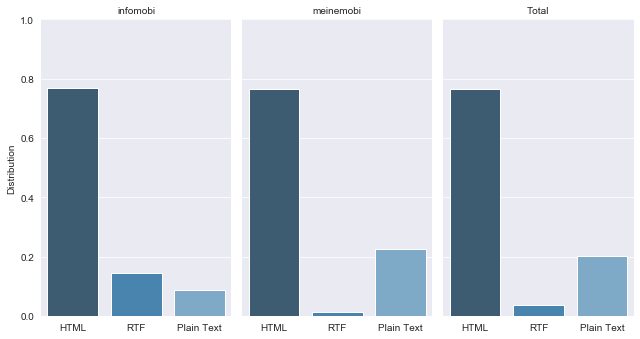
\includegraphics[scale=0.4]{plot-comparison-types}
    \caption{Distribution of the three message types}
    \label{fig:plot-comparison-types}
\end{figure}

Another important key figure is the typical length of a message. This key number can be measured in the total of words or characters. Figure \ref{fig:plot-comparison-words} shows that the statistical mean of words is 196.

The division of the number of characters by the amount of words provides an idea about the typical word in this specific context. Therefore the average word has a length of $8.45$ characters which is much higher than the average word in the \emph{Duden} corpus with its length of $6.09$ characters \cite{duden}. Possible reasons might be the formal language used in the business correspondence or insurance-related terms.

\begin{figure}[!ht]
    \begin{subfigure}{0.5\textwidth}
        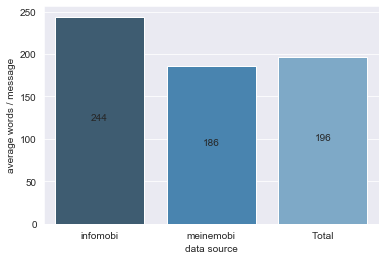
\includegraphics[scale=0.4]{plot-comparison-words}
        \caption{Comparison of words}
        \label{fig:plot-comparison-words}
    \end{subfigure}
    \begin{subfigure}{0.5\textwidth}
        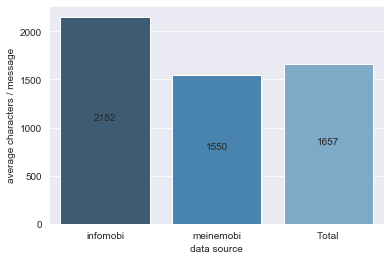
\includegraphics[scale=0.4]{plot-comparison-characters}
        \caption{Comparison of characters}
        \label{fig:plot-comparison-characters}
    \end{subfigure}
    \caption{Comparison of different indicators}
\end{figure}

\subsection{Typical Contents}
\label{chap:typical-contents}

Most messages can be divided into different groups. Such groups come very handy at the cleansing stage when patterns should be found to locate and remove junk from the remaining information. Therefore the \emph{mobi24} data can be splitted into several groups which are best described with sample messages.

\subsubsection{Spam and Junk}

Junk mails are much harder to detect today than they used to be in the past. Nowadays they are well written and mostly grammatically correct. Basically you could even use spam to train your model for certain use cases. But in that case spam should consistently be removed from the data set because it lacks of the insurance context which the model should get familiar with. The presence of links, the message length and the used language are often good indicators for detecting spam, especially when multiple indicators occur together.

\begin{quote}
    "Ein Ding der Unmöglichkeit! https://zixiseren1983.blogspot.in Auf Wiedersehen Elisabeth Speck"
\end{quote}

\begin{quote}
    "Mit der richtigen Haarpflege zur Traummähne :-) Die besten Pflegeprodukte für jeden Haartyp Endlich schöne Haare! Es ist Zeit, neue Haarprodukte zu entdecken..."
\end{quote}

\subsubsection{Auto-Generated Messages}

Some messages may not origin from real people but from machines instead. These group of messages is called \emph{automatically generated} and represents the largest group of messages an usual human receives per day. In the data source there are newsletters, notifications like payment success or delivery messages and failure reports present.

\begin{quote}
    "Fehler bei der Nachrichtenzustellung an folgende Empfänger oder Gruppen: generated1414@mobi.ch Die eingegebene E-Mail-Adresse konnte nicht gefunden werden..."
\end{quote}

\subsubsection{Customer Messages}

Moving forward, the messages which are actually written by humans and target Swiss Mobiliar's businesses are the only relevant ones for the model. There's a wide range of message types like sponsoring requests, claim notifications, and technical questions. All these messages share the same context.

Email messages are not as formal as letters and sometimes contain spelling errors. The texts are covered with typical Swiss expressions. There are even Swiss Mobiliar specific words like the name of products, magazines or applications. It's important to train the future model on this data to let it become aware of this typical kind of language.

\begin{quote}
    "Geschätzte Mobiliar ich habe mein Passwort verlegt. mit flotten Grüssen H. Muster"
\end{quote}

\begin{quote}
    "Guten Tag Im Anhang sende ich Ihnen die Offerte zum Schadenfall 8002.2533.9/XX zu. Wir bitten Sie die Offerte zu prüfen. Freundliche Grüsse Fritz Fischer"
\end{quote}

\section{Collecting Data}

As mentioned in \ref{chap:data-source}, the source data is stored in two separate PST files. To extract information from this proprietary file format a library called \emph{pypff}\footnote{Available at \url{https://github.com/libyal/libpff/wiki/Python-development}} is used. The email messages are stored in different directories which can have multiple sub-folders inside. Because of this structure, a recursive approach is needed to collect the data. Listing \ref{code:traverse} shows the detailed implementation including the calls to parse (:8) and clean (:10) the messages at the same iteration. The parser consists of three independent routines to get the message string from HTML, RTF, and plain text emails. The cleansing procedure is explained in the next section.

\begin{lstlisting}[language=Python, label={code:traverse}, caption=Recursively traversation of email folders]
def traverse(folder, mails):
    """ Recursively traverses a folder and collects all messages """

    # iterate over all messages in current folder
    for i in range(folder.get_number_of_sub_messages()):
        _message = folder.get_sub_message(i)

        message = parse(_message)

        message['text'] = clean_data(message['text'])

        if message and message['text']:
            mails = mails.append(message, ignore_index=True)

    # iterate over all sub folders
    for j in range(folder.get_number_of_sub_folders()):
        subfolder = folder.get_sub_folder(j)
        mails = traverse(subfolder, mails)

    return mails
\end{lstlisting}

\section{Data Cleansing}
\label{chap:cleansing}

As seen in section \ref{chap:typical-contents} there is a huge part of messages which shouldn't be used for further processing. These messages should be cleared from the message pool. This discipline is called data cleansing and can save a lot of time later in the project if it's done carefully. However, not all messages need to be removed completely from the data set. There exist a few cases where it's possible to only remove certain pieces of a message like signatures or the forwarded parts which are added by default if you reply to an e-mail.

Listing \ref{code:regular-expressions} shows a sample of the used regular expressions to detect unwanted content within the messages. If a junk pattern (:1-3) matches, the whole message is deleted. The forwarded parts of messages, which are often displayed as citations, are stripped off with several patterns (:5-10). The regular expressions come from observations during the exploration of the data sources.

\begin{lstlisting}[language=Python, label={code:regular-expressions}, caption=Regular expressions for junk detection]
JUNK_1 = re.compile('^Fehler bei der Nachrichtenzustellung')
JUNK_2 = re.compile('^Submitted on(.)*Submitted values are:')
JUNK_3 = re.compile('^Form Returned: Telefonnotiz')

FORW_1 = re.compile(r"[-]{5}\s*(Message d'origine)\s*[-]{5}")
FORW_2 = re.compile(r'[-]{5}\s*Weitergeleitete Nachricht\s*[-]{5}')
FORW_3 = re.compile(r'Am \d{2}.\d{2}.(20)?\d{2} (um )?\d{2}:\d{2}')
FORW_4 = re.compile('Von:(.)*An:|From:(.)*To:')
FORW_5 = re.compile('Submitted on(.)*Submitted values are:')
FORW_6 = re.compile('GB Digitaler Kundensupport <(.)*> schrieb am')
\end{lstlisting}

Further, the exploration showed that messages with a length of more than 3000 characters\footnote{The remaining length after stripping off signatures and forwarded parts} are principally newsletters or spam. On the other hand, messages with a remaining length of less than 75 characters aren't of interest either. Therefore only messages between these two boundaries are chosen for further processing steps.

The email messages are written mostly in German but some other languages like French, Italian, and English can be found too. The final model should be able to predict named entities in German but not in foreign languages which would require a lot more training data and knowledge about these languages. A data scientist at Swiss Mobiliar recently developed a library which combines four language recognition methods to predict the language of a given text by calling all four functions and returning the language with the most votes. This library has the appropriate name
\emph{LangVoter} and is used to filter out any non-German messages.

After data cleansing the number of messages is greatly reduced. More than 55 percent of messages have been removed (see Figure \ref{fig:plot-comparison-cleansing}). Figure \ref{fig:plot-comparison-cleansing-types} shows that the remaining data set consists of 10830 HTML (-48\%), 949 plain text (-83\%), and 378 RTF messages (-60\%). As mentioned in section \ref{chap:data-source} many auto-generated messages are of type RTF and plain text. Therefore it isn't surprising that most plain text and the bigger part of RTF messages don't contain valuable information for the training of a named-entity recognition.

A reliable deep learning model should be trained with as many samples as possible to give reasonable predictions. With a total amount of 12157 messages and the right techniques to virtually increase the training set size, this might be enough for the beginning. As you can see in chapter \ref{chap:sliding-window}, the sliding window technique is one solution to enlarge the training data without adding new samples.

\begin{figure}[ht!]
    \begin{subfigure}{0.5\textwidth}
        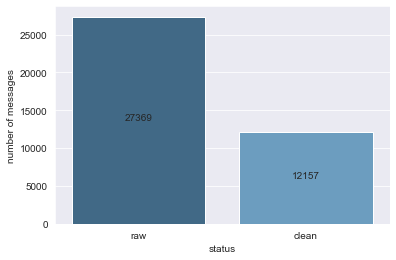
\includegraphics[scale=0.4]{plot-comparison-cleansing-total}
        \caption{Comparison in general}
        \label{fig:plot-comparison-cleansing}
    \end{subfigure}
    \begin{subfigure}{0.5\textwidth}
        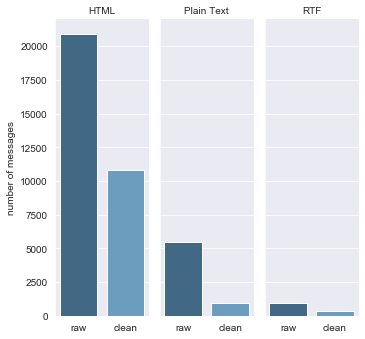
\includegraphics[scale=0.4]{plot-comparison-cleansing-type}
        \caption{Comparison grouped by type}
        \label{fig:plot-comparison-cleansing-types}
    \end{subfigure}
    \caption{Comparison before and after data cleansing}
\end{figure}

\section{Data Labelling}

In supervised learning a model needs to know the correct classification of the samples to compare them against its own predictions. The data set is called pre-labelled. An inevitable part of a data scientist's work is to label data manually. \emph{Doccano}\footnote{available at \url{https://doccano.herokuapp.com}} is an open-source text annotation tool built for creating labelled data. It supports sequence to sequence labelling which is useful for named-entity recognition.

\begin{figure}[!ht]
    \centering
    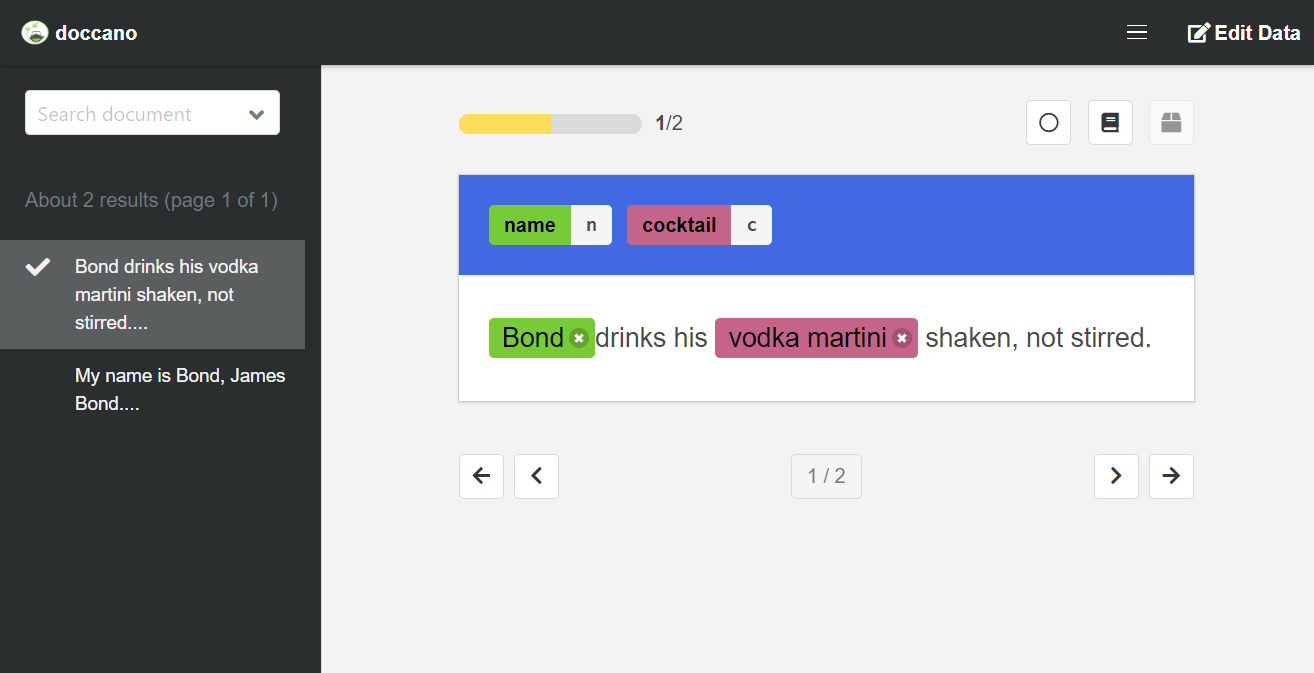
\includegraphics[scale=0.4]{doccano-example}
    \caption{Doccano annotation view}
    \label{fig:doccano-example}
\end{figure}

An advantage of \emph{Doccano} is the graphical user interface which helps you label data manually. You can even define shortcuts to speed up the labelling process.

\subsection{Doccano Parser}

One downside of Doccano are the limited options for exporting labelled data. You can download data only as JSON file with text labels. The exported file has the same structure as listing \ref{code:doccano-export}. If the exported data should be used as validation set it needs to become more handy to work with. Therefore I created a python library called \emph{mobi\_docparser}. The library allows users to parse Doccano's offset notation into a list with two elements: The text after a simple whitespace tokenisation and the corresponding labels for each token, either in IOB or binary notation. After parsing, the named-entity \emph{vodka martini} would be split into the tokens \emph{vodka} (B-DRINK) and \emph{martini} (I-DRINK).

\begin{lstlisting}[label={code:doccano-export}, caption=Sample export from Doccano as JSON (text labels)]
{
  "id": 12162,
  "text": "Bond drinks his vodka martini shaken, not stirred.",
  "meta": {},
  "annotation_approver": null,
  "labels": [[0, 4, "per"], [16, 29, "drink"]]
}
\end{lstlisting}

The offset notation defines named entities by their position inside the text. In the example above, the person entity \emph{Bond} starts at index \emph{0} and ends before index \emph{4}. It's very common in programming, that the second argument doesn't point at the ending token but at the token right after the marked sequence.

\subsection{Annotation Standards}

Named entities need to be described in a standardised way so that ML models can interpret them. There exist a few annotation standards which are often used in NER. If you have to chose a specific labelling standard, keep in mind that sophisticated labelling techniques give you more information than e.g. binary labelling. You can always downgrade to a lower standard but getting distinctive labels out of binary tags isn't possible. On the other hand, it's often easier to label data with low-level tags rather than e.g. IOB tags.

\subsubsection{Binary}

Binary tagging is the simplest form of labelling data. Every token which isn't a named entity is going to be labelled as 0. The remaining tokens which are all entities are tagged with 1. If multiple label types need to be distinguishable, binary tagging isn't the preferred method. As you can see in table \ref{tbl:binary-labelling}, the two entities \emph{people} and \emph{food} cannot be distinguished.

\begin{table}[h!]
    \centering
    \begin{tabular}{|c|c|c|c|c|c|c|c|}
        \hline
        Bond & drinks & his & vodka & martini & shaken, & not & stirred. \\
        \hline
        1 & 0 & 0 & 1 & 1 & 0 & 0 & 0 \\
        \hline
    \end{tabular}
    \caption{Example of a binary tagged sentence}
    \label{tbl:binary-labelling}
\end{table}

This issue can be solved by using multi-class labelling. This technique uses distinctive labels for every entity type as seen in \ref{tbl:multiclass-labelling}.

\begin{table}[h!]
    \centering
    \begin{tabular}{|c|c|c|c|c|c|c|c|}
        \hline
        Bond & drinks & his & vodka & martini & shaken, & not & stirred. \\
        \hline
        1 & 0 & 0 & 2 & 2 & 0 & 0 & 0 \\
        \hline
    \end{tabular}
    \caption{Example of multi-class tagged sentence}
    \label{tbl:multiclass-labelling}
\end{table}

\subsubsection{IOB (Inside-outside-beginning)}

Unlike binary tags, IOB labels allow you to differentiate between multiple label types. \emph{Bond} and \emph{vodka martini} are clearly not in the same entity group (\ref{tbl:iob-labelling}). Additional to the variable types, IOB tagging indicates multi-token entities as such. In the \emph{IOB2} format, the first token of a sequence is always labelled with the prefix \emph{B-} for beginning, the rest with an \emph{I-} for inside \cite{bio95}.

\begin{table}[h!]
    \centering
    \begin{tabular}{|c|c|c|c|c|c|c|c|}
        \hline
        Bond & drinks & his & vodka & martini & shaken, & not & stirred. \\
        \hline
        B-PER & O & O & B-FOOD & I-FOOD & O & O & O \\
        \hline
    \end{tabular}
    \caption{Example of an IOB tagged sentence}
    \label{tbl:iob-labelling}
\end{table}

As shown in table \ref{tbl:iob-labelling2}, the first two tokens are from the same type but still distinguishable. With binary tags you would most likely interpret both tokens as one large named entity consisting of two separate words.

\begin{table}[ht!]
    \centering
    \begin{tabular}{|c|c|c|c|c|c|}
        \hline
        Huey, & Dewey, & and & Louie & are & triplets. \\
        \hline
        B-PER & B-PER & O & B-PER & O & O \\
        \hline
    \end{tabular}
    \caption{Example of distinctive beginning tags}
    \label{tbl:iob-labelling2}
\end{table}

\subsubsection{BIOES}

The IOB format was later extended by an indicator for single and ending tokens. It's called \emph{BIOES} and can be useful if tokens are processed separately from each other so that the model cannot be able to recognise multi-token values by itself. The \emph{s} stands for single tokens whereas the \emph{e} indicates ending tokens \cite{hofer18}.

\begin{table}[h!]
    \centering
    \begin{tabular}{|c|c|c|c|c|c|c|c|}
        \hline
        Bond & drinks & his & vodka & martini & shaken, & not & stirred. \\
        \hline
        S-PER & O & O & B-FOOD & E-FOOD & O & O & O \\
        \hline
    \end{tabular}
    \caption{Example of an BIOES tagged sentence}
    \label{tbl:bioes-labelling}
\end{table}

\chapter{Baseline Models}

A baseline algorithm is a trivial approach to solve a certain task. It's common-sense-based and doesn't include any advanced data science techniques. They are simple to create, but often hard to beat. If the baseline can not get beaten by a high-sophisticated \acrshort{ml} model, the benefit of this model should be considered. For classification tasks with imbalanced data, it's nothing unusual to predict all samples with the label of the largest class \cite{rama18}.

\section{SpaCy Model}

SpaCy is meant to be the fast and easy-to-use \acrshort{nlp} library for the industry. Unlike more scientific libraries like NLTK\footnote{For more
information consider \url{https://www.nltk.org}}, spaCy focuses on getting work done rather than optimizing parameters to achieve even better results.
It's shipped with support for more than 53 languages including \acrlong{ner}, pretrained word vectors, and a non-destructive tokenization\footnote{
SpaCy's tokenization is fully reversible to reconstruct the original text} \cite{spacy}.

\subsection{Implementation}

As the developers of spaCy mentioned on their homepage, it's very easy to integrate spaCy into your project. With just a few lines of code a pretrained
language model can process input texts.

\begin{lstlisting}[language=Python, label={code:spacy-integration}, caption=Sample of a runnable spaCy model]
import spacy

# load the German language model
nlp = spacy.load('de_core_news_md')

# process text
doc = nlp('Bond drinks his vodka martini shaken, not stirred.')

for token in doc:
    # print named-entities
    print(token.ent_type_)
\end{lstlisting}

There exist three German language models which can be used to process text. As seen in listing \ref{code:spacy-integration} (line 4) the medium-sized
news model is used for this baseline approach. The model has a size of 214 MB and is able to recognise \emph{LOC}, \emph{MISC}, \emph{ORG}, and
\emph{PER} entities \cite{gh-spacy}. It's trained with data sources from the \emph{TIGER Corpus} and \emph{WikiNER}. The former has been trained with
approximately 50 000 sentences from the \emph{Frankfurter Rundschau} newspaper \cite{tiger}.

The \emph{WikiNER} corpus represents 7200 manually-labelled Wikipedia articles including the nine largest Wikipedias including English, German, Spanish,
and French. Unlike the \emph{TIGER Corpus}, the data quality of \emph{WikiNER} is only silver-standard. This means that the data is automatically created
by exploiting Wikipedia. Every internal link inside an article is getting replaced by the manually-labelled \acrshort{ne} category of the linked article \cite{Nothman}.

\subsection{Validation}

To validate spaCy's predictions the results need to be compared against the labelled \gls{mobi24} data. Because of the more sophisticated tokenisation
process of spaCy, the tokens aren't comparable with the output of the \emph{mobi\_docparser} library at first. By default, spaCy ignores the points in texts like \emph{Dr. House} or \emph{U.S.A} and doesn't treat the sequences as different sentences.

To get matching sets of tokens, spaCy's default tokenizer needs to be overwritten with a simple whitespace tokenizer.
As seen in listing \ref{code:tokenizer} the custom tokenizer simply uses the \verb|split()| function of
python's string module \cite{spacy-tok}.

\subsection{Performance}

Due to the fact that the model is trained on the \emph{TIGER} and \emph{WikiNER} corpus, it isn't very surprising that spaCy has it's difficulties with
recognising addresses because the corpora don't provide that many. SpaCy gets a mediocre \emph{f1 score} of \textbf{0.485}\footnote{Measured with the
current state of the labelling process (967 messages)}. As discussed in section \ref{chap:accuracy} the high accuracy of \textbf{0.946} shouldn't be used
as a performance indicator. The number of outside tokens compared to named entities is too imbalanced. For more information refer to table \ref{tbl:perf-spacy}.
If both entity types are considered separately, there is a huge gap between the \acrshort{kpi}s. As seen in tables \ref{tbl:perf-spacy-per} and
\ref{tbl:perf-spacy-loc}, recognising only names has a more than eight times higher \emph{f1 score} than address recognition. This leads to the assumption, that the German spaCy model haven't been trained on enough address data. 

If we have a closer look at the predictions spaCy did, we can see that many domain specific language is misinterpreted. Considering table
\ref{tbl:spacy-wrong-predictions}, domain language like \emph{\Gls{Protekta}} or \emph{Mobiliar} are recognised as named-entities of type \emph{PER}. Even
very common words like \emph{Hallo}, \emph{Lieber}, and \emph{Gruss} are falsely predicted. These kind of words occur often before names, which might be
a possible reason why spaCy has its problems with.

\begin{table}[h!]
    \centering
    \begin{tabular}{|C{6em}|L{25em}|}
        \hline
        \textbf{Prediction} & \textbf{Exampe Tokens} \\ [0.5ex]
        \hline
        PER & Protekta, Mobiliar, Initial-Passwort, Weihnachtstage, Telefongespräch, Hauptstrasse, Hallo, Lieber, Gruss, Danke \\ [0.5ex]
        \hline
        LOC & Kundenportal, Mobirama, Gebäudeversicherung, Webbrowser, www.mobiliar.ch/login, Sicherheitsgründen, Datenschutzgründen, Mobiltelefon \\ [1ex]
        \hline
    \end{tabular}
    \caption{Examples of false spaCy predictions}
    \label{tbl:spacy-wrong-predictions}
\end{table}

It's very irritating that spaCy predicts URLs as addresses. These tokens follow a specific pattern and could be easily recognised by a simple
regular expression. Unlike falsely predicted names, the most common mispredictions for addresses cannot be grouped together easily. The tokens are
often insurance related, but they seem to be distributed randomly.

\subsection{Conclusion}

SpaCy keeps what it promises. It's the easy-to-use library for processing texts. Within less than ten lines of code a fully working \acrlong{ner} can
be used to understand natural language. SpaCy's performance depends on the underlying model and data to be applied to. According to the official website the medium-sized German
model should achieve an overall \emph{f-score} of more than \textbf{0.834} \cite{spacy}. This score nearly doubles the score spaCy achieved while
processing the \gls{mobi24} data.

The library offers to do a retraining with an individual labelled corpus. This would make the model familiar with the insurance context. It's uncertain
how much the performance would improve. Due to limited time resources the spaCy approach isn't developed further. But the spaCy model can be used as a baseline model.

\section{Basic Lookup Model}
\label{chap:regex-model}
A written language consists of a word set and a rules set to describe how single words can be combined together to form larger constructs
like sentences or even texts. Every language follows a specific pattern which changes over time. In information technology, there exist
regular expressions\footnote{Patterns for defining character sequences used for search, replace or validation operations} which are very useful
to locate patterns inside text.

A basic implementation of a regular expression based algorithm for \acrlong{ner} may sound very costly if you have to define every language rule
as a regular expression. But it can be simplified by the use of reference data. This kind of data are called dictionaries and let you lookup
certain words to classify them according to the dictionary they are part of. This seems to be a very solid basis for classifying text. But because
of word ambiguity it's very important to define how to proceed if a term occurs in multiple dictionaries and not to simply rely on them.

\subsection{Basic Dictionary Lookup}

This basic approach starts with a simple dictionary lookup. Data scientists at Swiss Mobiliar created two dictionaries containing first and last names.
These lists are filled with a large amount of names due to different varieties of a single name and the different cultures people come from nowadays.
Together there are more than 140.000 names present.

\begin{lstlisting}[language=Python, label={code:regex-dict-lookup}, caption=Simple dictionary lookup]
import pandas as pd

first_names = pd.read_csv('./dictionaries/firstnames.csv', header=None, encoding='cp1252')[0]

def predict(token):
    if token in first_names:
        return 'PER'
    return 'O'
\end{lstlisting}

As seen in listing \ref{code:regex-dict-lookup}, the \emph{pandas} package is used to easily load data from the dictionary with a given encoding. \emph{CP-1252}
is an 8-bit encoding originally created for Microsoft Windows. Both name dictionaries are encoded with \emph{CP-1252}, sometimes also called \emph{ANSI}.

The dictionaries for addresses are manually created with data from the \emph{Federal Statistical Office} \cite{bfs}. There is a dictionary containing
all valid zip codes for Switzerland and another one with every municipality. Municipalities are stored in lowercase with escaped umlauts. This format
can be easily reproduced with just a few lines of python code. Another dictionary with a vast amount of street names is provided by another data scientist
at Swiss Mobiliar.

Table \ref{tbl:perf-regex} shows that the simple dictionary lookup approach only reaches an unpleasant precision of about \textbf{0.146}. Even with very
decent recall of \textbf{0.733}, the resulting \emph{f1-score} is \textbf{0.243}. The lookup model's precision is much lower compared to the German spaCy model,
which means that there are many falsely predicted tokens. An enhancement to the current model will focus on increasing its precision.

\subsection{Enhancements}

Some improvements need to be made to increase the \emph{f1-score} of the basic lookup model. Table \ref{tbl:perf-spacy} refers to the resulting performance indicators.

\subsubsection{Clean last names dictionary}

Checking false predictions shows that the last names dictionary contains many ambiguous values which are proper last names but have a different meaning in most scenarios.
The precision rises to a value nearly four times the original value if the last name lookup is being removed. Though the recall drops from \textbf{0.73} to \textbf{0.4}
because last names aren't recognised any longer. The optimal solution lies somewhere in between where many ambiguous values should be removed from the dictionary. But
this cleanup process will inevitably reduce the recall.

\begin{quote}
    "Herren, Weiss, Guten, Franken, Grund, Juli, Mobiliar, Mobi, Kunde"
\end{quote}

After removing ambiguous values the precision jumps from originally \textbf{0.146} to \textbf{0.432} with a minimal loss on recall of only \textbf{1\%}. There are
several terms which are obviously not names like \emph{Mobiliar}, \emph{Mobi}, or \emph{Kunde} which are removed too.

\subsubsection{Add a scoring scheme}

A match in the dictionary might not be enough to determine the token's entity type. Therefore a scoring system can be helpful to give each feature an individual score.
Names and addresses normally start with an uppercase letter. With these two conditions the model's precision increases to \textbf{0.487} with an unchanged
recall. 

\subsubsection{Compare against multiple variants}

Tokens might be all capital letters or without escaped umlauts or \gls{diacritic}s. It can be useful to lookup for several slightly modified versions of the original token. As
seen in table \ref{tbl:perf-regex} (rows 5/6), this enhancement lifts the \emph{f1-score} over \textbf{60\%}.

\begin{lstlisting}[language=Python, label={code:regex-variants}, caption=Creating different variants of a single token]
def create_variants(token):
    """
    Creates multiple variants of the same token for dictionary lookup
    """
    original = token
    cleaned = clean_token(token)
    small = umlauts.lower()
    umlauts = escape_umlauts(original)
    special = re.sub(r'[.,;:\-_]', '', small)
    diacritics = escape_diacritics(small)

    return {original, cleaned, small, umlauts, special, diacritics}
\end{lstlisting}

The newly created set of tokens can easily be compared with the dictionaries by using the \verb|intersection(t)| operation of the standard library.

\subsubsection{Involve the token's neighbours}

A valid address consists of several parts including the street name, street number, postal code, and municipality. Therefore these parts appear in a certain
sequence. After detecting a postal code in the previous processing loop there seems to be a significantly higher chance that a municipality will follow next.

Unfortunately there is no difference in recognising addresses. The \emph{f1-score} gains only \textbf{0.1\%} but the number of dictionary lookups nearly triples.
A possible reason might be, that there aren't that many addresses in the training and validation set. Due to this microscopic performance benefit and the extended
processing time, the changes are discarded.

\subsubsection{Naming dictionary clean up}

There are still many ambiguous tokens which are falsely predicted as names. After a more rigorous clean up of both naming dictionaries, the \emph{precision} climbs
from former \textbf{50.4\%} to pleasant \textbf{77.3\%}. This is done with a German stop words dictionary\footnote{Found online at
https://countwordsfree.com/stopwords/german} which values are intersected with the naming dictionaries. Every match is directly removed from the naming dictionaries.
Additionally the hand-crafted list of mostly ambiguous names (see listing \ref{lst:excluded-names}) is extended to 75 values in total.

\subsubsection{Replace address dictionary with regex}

After improving the \emph{precision} of recognising names, address recognition is still lousy. The address dictionary contains too many unreliable values. Some of
them are really ambiguous but many of them are clearly nonsense. The vast dictionary has a total size of 139 660 entries.

\begin{quote}
    "A1 Ausfahrt Raststätte Nord, ABC Kompetenzzentrum, Airport Shopping Center, Aktie, Chrome, Grunder, Kirche, Kleben"
\end{quote}

After replacing the dictionary lookup with a very basic regular expression (listing \ref{code:regex-address}), the \emph{precision} rises to \textbf{0.848} with only
a little decrease in \emph{recall}. This leads to an overall \emph{f1-score} of \textbf{78.6\%} which is pretty neat and challenging for a baseline algorithm.

\begin{lstlisting}[language=Python, label={code:regex-address}, caption=Very basic regular expression for detecting addresses]
re.search(r'^.{2,}(strasse|gasse|gaessli|weg)', token)
\end{lstlisting}

\subsection{Conclusion}

The basic lookup model performs much better than the spaCy solution. With a final \emph{precision} of \textbf{84.8\%} only 15 percent of its predictions are false. But
with a \emph{recall} of \textbf{73.2\%} the model doesn't recognise a third of all names and addresses. For this reason the model can be improved with even better
dictionaries, a more sophisticated scoring system, and superior regular expressions before using it in practice.

As visible in tables \ref{tbl:perf-regex-per} and \ref{tbl:perf-regex-loc} the basic lookup model has the same issues with address recognition as the spaCy model. Because of the
imbalanced data the very low \emph{f1-score} of \textbf{16.6\%} doesn't count much. Nevertheless a good working \acrlong{ner} should be able to recognise addresses
as well. Needless to say that the actual model totally ignores street numbers.

All in all, it's much harder to compete against the basic lookup model rather than the spaCy approach. The basic lookup model has a \emph{f1-score} of \textbf{78.6\%} which is much better than the \textbf{48.5\%} of the spaCy model. Therefore this is a great baseline which needs to be beaten by deep learning at first.

\chapter{Deep Learning}

An auspicious field of \acrlong{ml} is deep learning.

With the raise of graphic cards a concept from 1960 has become more interesting in recent years.

aims to overpower baseline approaches

\section{Defining Input and Output Layers}

Write why the input is important and why the network can calculate the other dimensions according to the used layers itself.

\subsection{Sliding Windows}
\label{chap:sliding-window}

Due to different lengths of the text samples, the input layer of the neural network cannot rely on the number of words in the corpus. It has to be consistent
throughout the whole training and validation process. One possible solution is to adjust the input dimension to the size of the longest sentence in the corpus,
but this would wastefully bloat the network's parameter space. Needless to say that this enormous structure is only used by the longest text and is an overhead
for all other input values. Another possibility is to use the \verb|pad_sequences()|\footnote{more information at https://keras.io/preprocessing/sequence} function
of \emph{Keras} which simply trims sentences to a specific length. Unfortunately many tokens at the end of texts will get cut off.

A well-constructed deep learning model shouldn't only rely on a single token to make its predictions. Especially in \acrshort{nlp} the context is fundamental for
making suitable predictions. Therefore the sliding window functionality comes in very handy. It creates multiple windows with of a defined length but with different
tokens. Every token of a text is at least once present in a window. Listing \ref{code:sliding-window} shows how these slices are generated.

Table \ref{tbl:sliding-window} illustrates the \verb|sliding_window()| function with an example. The colourized cell indicates the current token which the network
should predict. This single sentence results in eight windows. The sliding window technique duplicates the input data thus the original 967 sentences are split into
70354 windows of size 9.

\begin{table}[ht!]
    \centering
    \begin{tabular}{|c|c|c|c|c|c|c|c|c|}
        \hline
        \verb|i| & \multicolumn{7}{c|}{\textbf{Sliding Window}} \\ [0.5ex]
        \hline
        1 &  &  &  & \cellcolor[HTML]{eaeaf2} Bond & drinks & his & vodka \\ [0.5ex]
        \hline
        2 &  &  & Bond & \cellcolor[HTML]{eaeaf2} drinks & his & vodka & martini \\ [0.5ex]
        \hline
        3 &  & Bond & drinks & \cellcolor[HTML]{eaeaf2} his & vodka & martini & shaken, \\ [0.5ex]
        \hline
        4 & Bond & drinks & his & \cellcolor[HTML]{eaeaf2} vodka & martini & shaken, & not \\ [0.5ex]
        \hline
        5 & drinks & his & vodka & \cellcolor[HTML]{eaeaf2} martini & shaken, & not & stirred. \\ [0.5ex]
        \hline
        6 & his & vodka & martini & \cellcolor[HTML]{eaeaf2} shaken, & not & stirred. & \\ [0.5ex]
        \hline
        7 & vodka & martini & shaken, & \cellcolor[HTML]{eaeaf2} not & stirred. &  & \\ [0.5ex]
        \hline
        8 & martini & shaken, & not & \cellcolor[HTML]{eaeaf2} stirred. &  &  & \\ [0.5ex]
        \hline
    \end{tabular}
    \caption{Sliding windows of size 7}
    \label{tbl:sliding-window}
\end{table}

\subsection{Using Keras Tokenizer}

The input into a neural network has to be numeric. Therefore a very simple solution is to map every word to an unique ID. The \emph{Keras tokenizer} creates an ID for
every distinctive word in the training data. As seen in table \ref{tbl:keras-tokenizer} the IDs are ranked by their frequency in the text. The words \emph{to} and
\emph{be} are more frequent than the rest so they have got a lower ID.

\begin{table}[ht!]
    \centering
    \begin{tabular}{|l|c|c|c|c|c|c|c|c|c|c|}
        \hline
        \textbf{Original} & To & be, & or & not & to & be, & that & is & the & question. \\
        \hline
        \textbf{Tokenized} & 2 & 3 & 4 & 5 & 2 & 3 & 6 & 7 & 8 & 9 \\
        \hline
    \end{tabular}
    \caption{Example output of the Keras tokenizer}
    \label{tbl:keras-tokenizer}
\end{table}

The first ID is reserved for a special token called \emph{OOV} (out-of-vocabulary). You have to fit the tokenizer on a given text which may not contain the same
tokens than the test set. Every word which the \emph{tokenizer} hasn't seen before gets labelled as \emph{OOV}. Consider listing \ref{code:keras-tokenizer} to see
how the tokenizer is being used.

\subsubsection{Vocabulary}

Normally the tokenizer's vocabulary only consists of the tokens in the training set to emulate a real world scenario for the model. Because of language changes or
misspelled words, unknown tokens aren't rare. Due to the sliding window technique, the input data gets multiplied by a factor of the exact window size. Therefore
even a token which only occurs once in the whole data exists now several times. The \verb|train_test_split()| will most likely add at least one instance of this
token to the train set. Multiple experiments confirm, that the tokenizer's word index contains more than 95\% of the vocabulary. It's a small flaw in the
architecture, hence the model would perform slightly worse in production.

\subsubsection{Disadvantages}

The main downside of using a tokenizer is that the IDs doesn't provide any additional information about the token itself. For example the Swiss German word \emph{Velo},
which means bicycle, is probably more frequently used in the corpus than the German version \emph{Fahrrad}. These two words share a very strong similarity but this
relation is invisible when using IDs. Therefore \emph{embeddings} should be used as described in section \ref{embeddings-chapter-here}.

\subsection{Output Layer}

To classify all tokens into the three classes \emph{O}, \emph{PER}, and \emph{LOC}, several solutions are applicable. Rather than getting a single neuron as output I
chose to use three output neurons where all are representing a class. 

\section{Building the first Network}

\section{Enlarging the Network}

more units, more fun

\section{Implementing Class Weights}

\subsection{Calculate Weights with Scikit-learn}

\subsection{Set Weights out of the stomach}

\section{Using Embeddings}

\subsection{Create own Embeddings}

\subsection{Use Wikipedia Embeddings}

\section{Define a Recurrent Neural Network}

\chapter{Summary}

The last chapter of this bachelor thesis focuses on reviewing the project and summarising the findings. It reveals what happens next with the deep learning model and how it could be further optimised.

\section{Reflection}

For humans it might be irritating to understand the issues computers can have in understanding natural language. After dealing with my own pre-processed data for more than four months, I can totally understand these poor little robots. Language is very versatile, ambiguous and even flexible, especially if humans don't pay too much attention on spelling.
After developing the baseline lookup model, I was worried about its respectable performance and if I was able to beat it with deep learning. Loosing against the baseline wouldn't devalue this bachelor thesis, but definitely hurt my pride as a data scientist.

\subsection{Lessons Learned}

During the last months I learned a lot about data science. I appreciate these lessons learned and think that mistakes you make are much more valuable than simply reading about experiences from others. As mentioned in section \ref{chap:deep-performance}, it is a bit devastating that things you learnt in theory don't apply in practice. This gave me an important insight about the work as a data scientist. You have to consider every problem individually. There is no such thing as a one-size-fits-all solution. It's often challenging to find answers about why an established concept works or doesn't work with my data.

I saw how time-consuming data cleansing can be. I have read several articles on this subject that said that data preprocessing takes up to 80\% of a data scientist's time, but I could not imagine this is true \cite{naman18}. After spending more than one month with preprocessing tasks I have to reconsider. I learned that a sound database is key to work with. In the first hour of data labelling, I didn't come across a single message containing junk, spam or any foreign language. This strengthened my belief that I did a good job at cleansing.

One aspect I totally underestimated was the performance measuring. Because of my previous classes I was aware of the existing key performance indicators and how to use them. Therefore, after creating the model I thought a simple part would begin. But I was wrong and performance measuring is not trivial. The test data needs to be in different shapes. For a model working with embeddings you have to map the test data also to word vectors. For the tokenised models the input needs to be tokenised and split into windows. You even have to define what happens if a model recognises a token as named entity \emph{LOC} but it's actually \emph{PER}. I decided to handle these situations as false positives\footnote{For the missed out \emph{PER}, a false negative would be correct too}.

In a future project, I would definitely spend less time in refactoring code for exploratory tasks which doesn't need to be robust. Exploring data is a very agile and fast task. I could have spent less time on these works if I didn't parameterise every piece of code or tried to generalise methods. Sometimes my experience as a software developer gets in my way when doing data science. On the other hand I'm very glad that I know how to develop software. Due to my knowledge it was very simple to release code in form of python libraries or work with the \emph{teamcity} build server.

\subsection{Motivation}

While working on this bachelor thesis there have been multiple key moments which kept me motivated. A very surprising aspect was, that I started to like labelling data. Many colleagues told me, it's a Sisyphean task which every data scientist has to do from time to time. I labelled my data in shifts and not more than one hour per session. I used this not so demanding work to make a pause or to get a distance between my mind and the work I've done before. This was especially useful when I was struggling with programming issues or couldn't think of a solution to a certain problem. Many times I returned to the previous task and had a bunch of new ideas what to try next.

A very motivating fact was, that I could act as a test user for my scrum team while progressing on my project. There were several test cases where my model or the data I used have been involved. I gave feedback to the so-called model project, which is basically a template that allows data scientist to deploy their models for using at Swiss Mobiliar. I uploaded my original data, the cleansed, and the labelled version of it to the data repository. The data repository is a self-made tool which allows sharing and versioning of data sets.

The baseline's performance maybe pushed me the most to develop an even better deep learning model. First I thought it was very challenging, but with the use of embeddings I overpowered the dictionary lookup model at first try. Seeing your model growing and increasing its performance is very exciting.

\section{Further Improvements}

After finishing this bachelor thesis, the NER project at Swiss Mobiliar doesn't end. There is a lot of work to do, before the model can be used in production. And there are some very promising concepts which I couldn't find the time to try out yet.

\subsection{Expand the Data}

I had to deal with a lot of overfitting. The best solution for this problem is to increase the training data size. But getting reliable data is one of the toughest problems in data science. Luckily one of the data scientists at Swiss Mobiliar is currently testing external labelling partners. For demonstration purposes they label several hundred messages of the \emph{Mobi24} dataset. If the data passes the gold standard, it will be used for training. A possible partnership with the company could result in much more data which would hopefully improve the generalisation capabilities of the model.

\subsection{Add Recurrent Layers}

The used multi-layer perceptron is a simple feed forward network. The neurons pass their data to the neurons in the next layer. Recurrent neural networks (RNN) are different to feed forward networks. Their neurons can be connected to neurons in the same or previous layer. This allows the network to process sequences with a given context. This is appreciated in tasks like speech recognition and especially natural language processing \cite{wiki07}. A specific RNN architecture, using a memory called \emph{cell state}, is the long short-term memory (LSTM). This memory helps keeping a relation between previous and next elements in a sequence. More information and the three gates used by a LSTM network are best described in its original paper of 1997 \cite{lstm97}. It is very promising that the use of recurrent layers will increase the model's performance. Due to limited time resources this will be tried out after the bachelor thesis ends.

\section{Acknowledgements}

I'd like to express my gratitude to my supervising professor Dr. Jürgen Vogel and the expert Pierre-Yves Voirol for keeping the project and especially this report on track. Special thanks to my supervisor at Swiss Mobiliar, Marcus Schwemmle, for his support during the last few months. I'm very happy that he and the other data scientists shared their vast knowledge with me.


% glossary
% \printglossaries

% bibliography
\bibliographystyle{plain}
\bibliography{references}

% appendix
\appendix
\chapter{Resources}

This chapter contains code snippets, performance measurements, and additional information which would unnecessarily bloat the report. Only the important parts are covered in this section. The complete source code was handed to the supervising professor before the submission deadline.

\section{Performance Metrics}

The \acrlong{kpi}s are measured with a total of 967 manually-labelled messages. These numbers will be affected by adding more trainig samples. Consider section \ref{chap:formulas} for more information about the different \acrshort{kpi}s.

\subsection{SpaCy}

\begin{table}[ht!]
    \centering
    \begin{tabular}{|p{6em}|p{3em}|}
        \hline
        Accuracy & 0.946 \\
        \hline
        Precision & 0.444 \\
        \hline
        Recall & 0.533 \\
        \hline
        \textbf{F1 Score} & \textbf{0.485} \\
        \hline
    \end{tabular}
    \caption{Spacy KPIs}
    \label{tbl:perf-spacy}
\end{table}

\begin{table}[ht!]
    \begin{minipage}{.5\linewidth}
        \centering
        \begin{tabular}{|p{6em}|p{3em}|}
            \hline
            Accuracy & 0.955 \\
            \hline
            Precision & 0.405 \\
            \hline
            Recall & 0.685 \\
            \hline
            \textbf{F1 Score} & \textbf{0.509} \\
            \hline
        \end{tabular}
        \caption{Spacy (only PER)}
        \label{tbl:perf-spacy-per}
    \end{minipage}%
    \begin{minipage}{.5\linewidth}
        \centering
        \begin{tabular}{|p{6em}|p{3em}|}
            \hline
            Accuracy & 0.933 \\
            \hline
            Precision & 0.039 \\
            \hline
            Recall & 0.158 \\
            \hline
            \textbf{F1 Score} & \textbf{0.063} \\
            \hline
        \end{tabular}
        \caption{Spacy (only LOC)}
        \label{tbl:perf-spacy-loc}
    \end{minipage}
\end{table}

\subsection{Basic Lookup Model}

Consider chapter \ref{chap:regex-model} for more information about the different enhancements.

\begin{table}[ht]
    \centering
    \begin{tabular}{|L{16em}|C{3em}|C{3em}|C{3em}|C{3em}|}
        \hline
        \textbf{Enhancement} & \textbf{Acc} & \textbf{Prec} & \textbf{Rec} & \textbf{F1} \\ [1ex]
        \hline
        1 - Add dictionary lookup & 0.774 & 0.146 & 0.733 & 0.243 \\ [0.2ex]
        \hline
        2 - Remove last names dictionary & 0.953 & 0.582 & 0.401 & 0.475 \\ [0.2ex]
        \hline
        3 - Clean up last names & 0.948 & 0.432 & 0.723 & 0.541 \\ [0.2ex]
        \hline
        4 - Add uppercase constraint & 0.953 & 0.487 & 0.722 & 0.582 \\ [0.2ex]
        \hline
        5 - Escape \gls{diacritic}s & 0.953 & 0.486 & 0.736 & 0.585 \\ [0.2ex]
        \hline
        6 - Add variants (e.g. umlauts) & 0.952 & 0.503 & 0.758 & 0.605 \\ [0.2ex]
        \hline
        7 - Add previous and next tokens & 0.954 & 0.504 & 0.761 & 0.606 \\ [0.2ex]
        \hline
        8 - Clean up first- and last names & 0.982 & 0.773 & 0.752 & 0.762 \\ [0.2ex]
        \hline
        9 - Replace addresses with regex & 0.98 & 0.848 & 0.732 & \textbf{0.786} \\ [0.2ex]
        \hline
    \end{tabular}
    \caption{Basic Lookup Model KPIs}
    \label{tbl:perf-regex}
\end{table}

\begin{table}[ht!]
    \begin{minipage}{.5\linewidth}
        \centering
        \begin{tabular}{|p{6em}|p{3em}|}
            \hline
            Accuracy & 0.984 \\
            \hline
            Precision & 0.737 \\
            \hline
            Recall & 0.885 \\
            \hline
            \textbf{F1 Score} & \textbf{0.804} \\
            \hline
        \end{tabular}
        \caption{Lookup Model (PER)}
        \label{tbl:perf-regex-per}
    \end{minipage}%
    \begin{minipage}{.5\linewidth}
        \centering
        \begin{tabular}{|p{6em}|p{3em}|}
            \hline
            Accuracy & 0.951 \\
            \hline
            Precision & 0.111 \\
            \hline
            Recall & 0.334 \\
            \hline
            \textbf{F1 Score} & \textbf{0.166} \\
            \hline
        \end{tabular}
        \caption{Lookup Model (LOC)}
        \label{tbl:perf-regex-loc}
    \end{minipage}
\end{table}

\subsection{Deep Learning}

Here are the metrics for the very deep net and stuff..

\section{Source Code}

\subsection{Keras Tokenizer}

The Keras tokenizer allows you to define the \emph{OOV} token during initialisation. With the \verb|filter| option you can define which characters the tokenizer should filter from the tokens. The default filter would handle "\emph{Hello}" and "\emph{Hello,}" as the same token. For not losing punctuation the \verb|filter| parameter needs to be set to an empty string.

\begin{lstlisting}[language=Python, label={code:keras-tokenizer}, caption=Fitting the Keras tokenizer]
from tensorflow.keras.preprocessing.text import Tokenizer

tokenizer = Tokenizer(oov_token='<OOV>', filters='')

# create a vocabulary based on the training set
tokenizer.fit_on_texts(train_sentences)

# create sequences of IDs
sequences = tokenizer.texts_to_sequences(test_sentences)
\end{lstlisting}

\subsection{Sliding Window}

\begin{lstlisting}[language=Python, label={code:sliding-window}, caption=Sliding window implementation]
def sliding_window(sequences, window_size=5, placeholder='', flatten=True):
    """
    Creates windows of the exact same size, first and last windows
    will be padded with a placeholder. The relevant token of each
    window is placed in the middle. Flattens the list by default.
    """
    half = int(window_size / 2)
    results = []

    for sequence in sequences:

        tokens = sequence[0]
        labels = sequence[1]

        length = len(tokens)
        windows = []

        # create windows
        for idx in range(length):
            start = idx - half
            stop = idx + 1 + half
            windows.append([tokens[max(0, start):stop], labels[idx]])

        # add padding for first windows
        for idx, val in enumerate(range(half, 0, -1)):
            tmp = windows[idx][0]
            for i in range(val):
                tmp = [placeholder] + tmp

            windows[idx][0] = tmp

        # add padding for last windows
        for val, idx in enumerate(range(length-half, length)):
            tmp = windows[idx][0]
            for i in range(val+1):
                tmp = tmp + [placeholder]

            windows[idx][0] = tmp

        results.append(windows)

    if flatten:
        results = [item for sublist in results for item in sublist]

    return results
\end{lstlisting}

\section{Miscellaneous}

\subsection{Excluded Ambiguous Names}
\label{lst:excluded-names}

The following list shows all values which aren't common names or which may be names but are ambiguous. These values are removed from the naming dictionaries which are used by the regex baseline model.

\begin{multicols}{4}
    \begin{itemize}
        \item mobiliar
        \item mobi
        \item immobilien
        \item safari
        \item franken
        \item guten
        \item leider
        \item min
        \item link
        \item weiss
        \item herr
        \item app
        \item kunde
        \item dame
        \item damen
        \item frau
        \item gerne
        \item sport
        \item firma
        \item herren
        \item liebe
        \item schaden
        \item grund
        \item person
        \item kinder
        \item mio
        \item juni
        \item bern
        \item mail
        \item post
        \item mar
        \item sun
        \item fall
        \item ort
        \item hand
        \item mon
        \item wed
        \item may
        \item gruss
        \item abend
        \item mai
        \item juni
        \item juli
        \item phone
        \item spray
        \item buchung
        \item freitag
        \item montag
        \item monday
        \item fehler
        \item glueck
        \item uri
        \item seite
        \item auto
        \item pin
        \item biel
        \item you
        \item helvetia
        \item weg
        \item art
        \item termine
        \item chance
        \item merci
        \item stecker
        \item preis
        \item partner
        \item restaurant
        \item handy
        \item zurich
        \item schlechten
        \item privat
        \item frische
        \item kan
        \item name
    \end{itemize}
\end{multicols}



\end{document}
